\chapter{问题描述}

\section{网络与故障模型}
考虑由 $n$ 个节点构成的有向通信图 $G(\mathcal{V},\mathcal{E})$，其中 $\mathcal{V}=\{1,\dots,n\}$ 为节点集合，$\mathcal{E}$ 为有向边集合。网络中未知的拜占庭节点子集记为 $\mathcal{A}$，其规模满足 $|\mathcal{A}|\le b$，$b$ 为系统预设的最大容忍故障数。记实际故障数 $\phi\triangleq|\mathcal{A}|$，则 $\phi\le b$。为保证算法可行性，限定 $n\ge 3b+1$。对每个节点 $i$，用 $\mathcal{N}_i$ 表示其入度邻居集合，入度 $d_i\triangleq|\mathcal{N}_i|$（图中不含自环，即 $(i,i)\notin\mathcal{E}$）。

采用标准拜占庭故障模型\upcite{lynch1996distributed}：恶意节点掌握全网信息，可任意偏离协议，且能对不同邻居发送不一致消息。例如，拜占庭节点 $i\in\mathcal{A}$ 在第 $t$ 轮发送给诚实节点 $j\in\mathcal{V}\setminus\mathcal{A}$ 的消息记为 $m_{ij}[t]$，则允许存在 $m_{ij}[t]\ne m_{ij'}[t]$（其中 $j\ne j'$，均为诚实节点）。

\section{拜占庭抗性优化目标}
令可行域 $\mathcal{X}\subseteq\mathbb{R}$ 为非空闭凸集。每个节点 $i$ 的局部代价函数 $f_i:\mathcal{X}\to\mathbb{R}$ 满足凸性、连续可微、$L$-Lipschitz 连续梯度，且其最优解集非空紧致。

无故障时，系统求解 $\min_x \frac{1}{n}\sum_{i=1}^{n} f_i(x)$，即所有节点权重均为 $1/n$ 的算术平均\upcite{tsianos2012,nedic2015}。但拜占庭节点可伪造 $f_i$，使该目标失效。为此，给定参数 $(\beta,\gamma)$（$\beta\in(0,1)$，$\gamma\in\mathbb{N}$），诚实节点寻求输出 $\widetilde{x}$ 满足
\begin{equation}
\widetilde{x}\in\arg\min_{x\in\mathcal{X}}\sum_{i\in\mathcal{V}\setminus\mathcal{A}}\alpha_i f_i(x),
\label{eq:robust}
\end{equation}
其中 $\mathcal{V}\setminus\mathcal{A}$ 表示诚实节点集合。权重系数 $\alpha_i$ 需满足
\begin{equation}
\alpha_i\ge0,\quad \sum_{i\in\mathcal{V}\setminus\mathcal{A}}\alpha_i=1,\quad
\sum_{i\in\mathcal{V}\setminus\mathcal{A}}\mathbf{1}\{\alpha_i\ge\beta\}\ge\gamma,
\label{eq:admissibility}
\end{equation}
这里 $\mathbf{1}\{\cdot\}$ 为指示函数（条件成立取1，否则取0）。条件 \eqref{eq:admissibility} 定义了权重向量 $\boldsymbol{\alpha}=[\alpha_1,\dots,\alpha_n]^\top$ 的 $(\beta,\gamma)$-可容许性：至少 $\gamma$ 个诚实节点的权重不低于 $\beta$，从而保证足够多节点的有效信息参与决策\upcite{charikar2017}。

然而，并非任意 $(\beta,\gamma)$ 都能实现，存在理论极限\upcite{su2016limits}：对任意 $\beta>0$，不可能保证存在满足 $\gamma>|\mathcal{V}\setminus\mathcal{A}|-b$ 的可容许权重。

为求解 \eqref{eq:robust}，本文提出双重修剪分布式梯度下降算法（见图\ref{fig:example}）。该算法通过在局部状态估计和局部梯度计算两个维度上同时执行极值截断筛选的操作，将含有对抗注入的非线性状态演化等效地约束在诚实节点的凸包内部，避免了拜占庭节点对正常节点的极端值攻击，同时更新时通过求均值和求最大最小值均值的方式分别得到更新后的局部值和梯度值，并采用投影的方式避免更新后的局部值偏离出合法安全解集，并且通过不断地迭代使最终的结果落入合法安全解集内。理论分析表明，在确保通信图满足约简图连通假设的前提下，该方法能够在牺牲一定寻优精度的条件下，保障系统在对抗环境中向合法目标解集渐近收敛。

\begin{figure}[h]
    \centering
    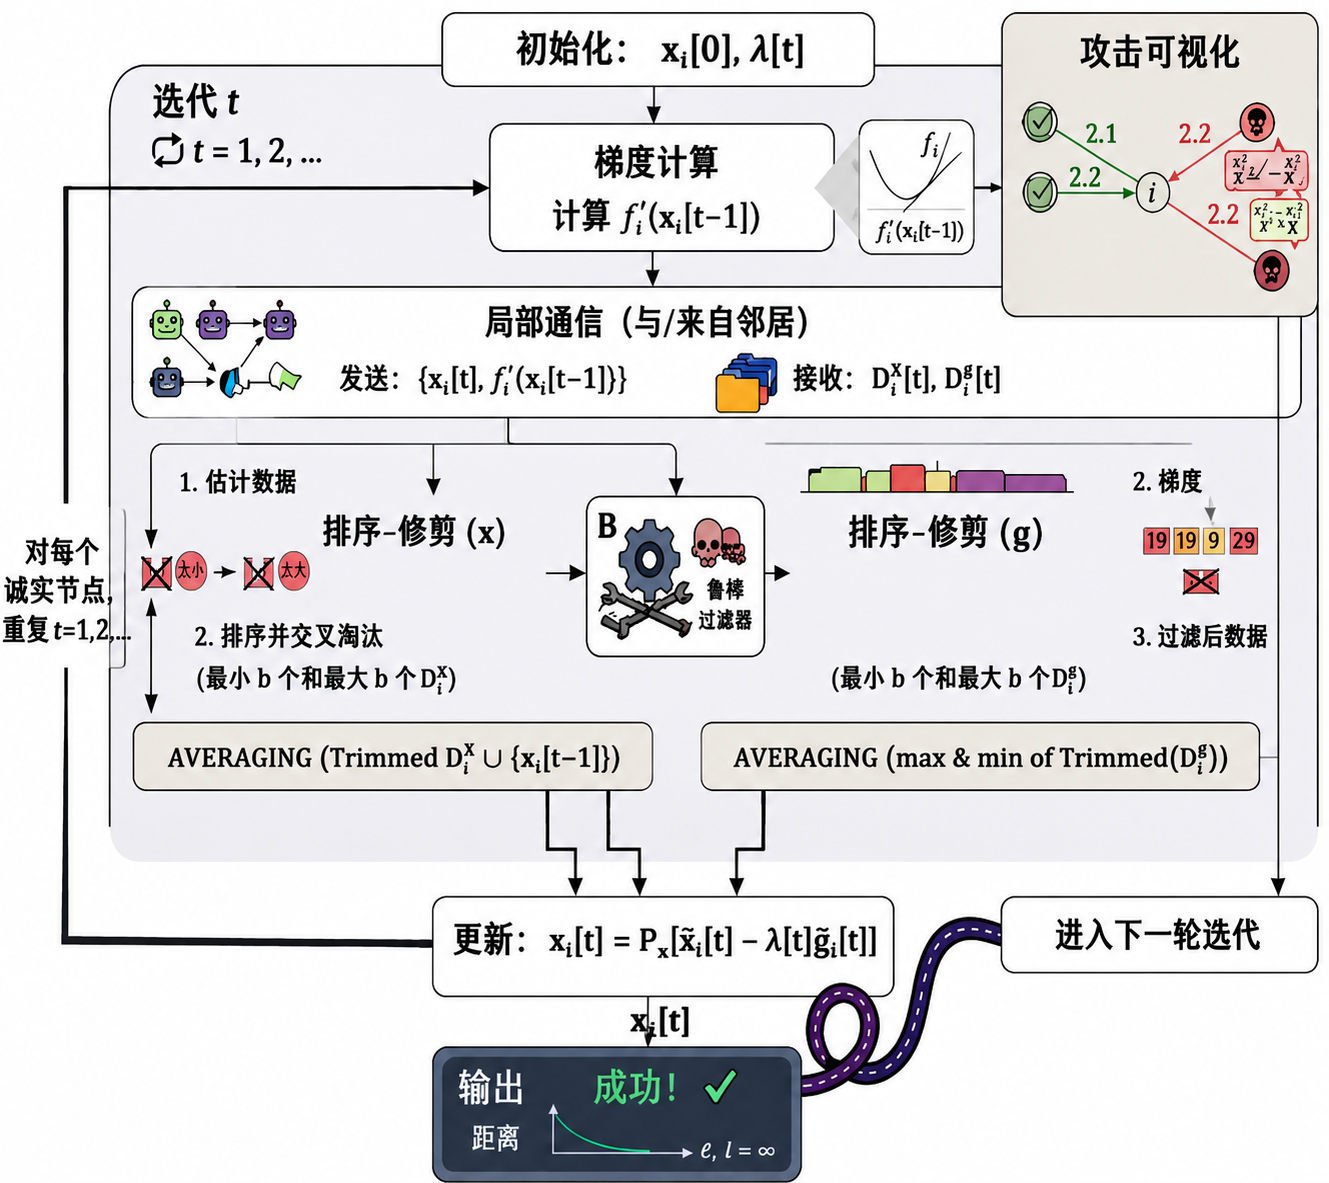
\includegraphics[width=0.8\textwidth]{function.png}
    \caption{基于双重修剪的分布式梯度下降算法图}
    \label{fig:example}
\end{figure}